\subsection{Design and construction of Mebench}
Evaluating models’ ability to identify and reason about regulatory mechanisms requires reference annotations that specify how a TF regulates its target gene and document the supporting experimental evidence. We therefore curated TF–gene relationships from published experimental studies. Each entry describes the TF–gene pair, its regulatory mechanism, and the evidence supporting that mechanism. The record includes validated contexts, references and source locations, the key feature required for the assigned mechanism category, mediator information and checks against all four candidate mechanisms (Figure~\ref{fig:benchmark_overview}).

The direct cis-regulatory DNA category requires TF occupancy at a promoter, enhancer or other cis-regulatory element linked to the target gene, together with functional evidence of TF-dependent target regulation. Functional evidence may come from perturbing either the TF or the regulatory element; the element itself need not be perturbed in every case. Occupancy, motif presence or an expression association alone is insufficient. Pairs are excluded if experimentally demonstrated dependencies meet the criteria for one of the other three categories. Chromatin-mediated regulation requires a specified chromatin state, modification, nucleosome process, or regulator whose necessity for TF occupancy, TF-dependent cis-regulatory activity, or the TF-dependent target response is demonstrated by perturbation, rescue, or an equivalent dependency test. Correlated accessibility or histone-mark changes do not alone establish this label. Combinatorial TF regulation requires a specified partner TF whose cooperation, competition, or antagonism is necessary for the target response, supported by individual or joint perturbation, interaction disruption, rescue, or an equivalent functional test. Regulatory RNA-mediated regulation requires a TF-to-RNA-to-target relay involving a named miRNA or lncRNA. The specified admission criteria require support for both links and the intermediate’s necessity through perturbation, rescue, or an equivalent dependency test. This regulation can affect RNA stability or translation. We therefore assign response labels according to the target-expression readout measured in the source study. After confirming the regulatory mechanism for each pair, we matched perturbation experiments conducted in compatible experimental contexts, with clearly defined perturbation–control comparisons and unambiguous measured responses of the target gene. The direction of change in target gene expression was defined relative to the corresponding control. The released source table contains the perturbation records. We also recorded the experimental methods, control conditions, doses, time points, assays and source locations. 
\begin{figure}[!t]
  \centering
  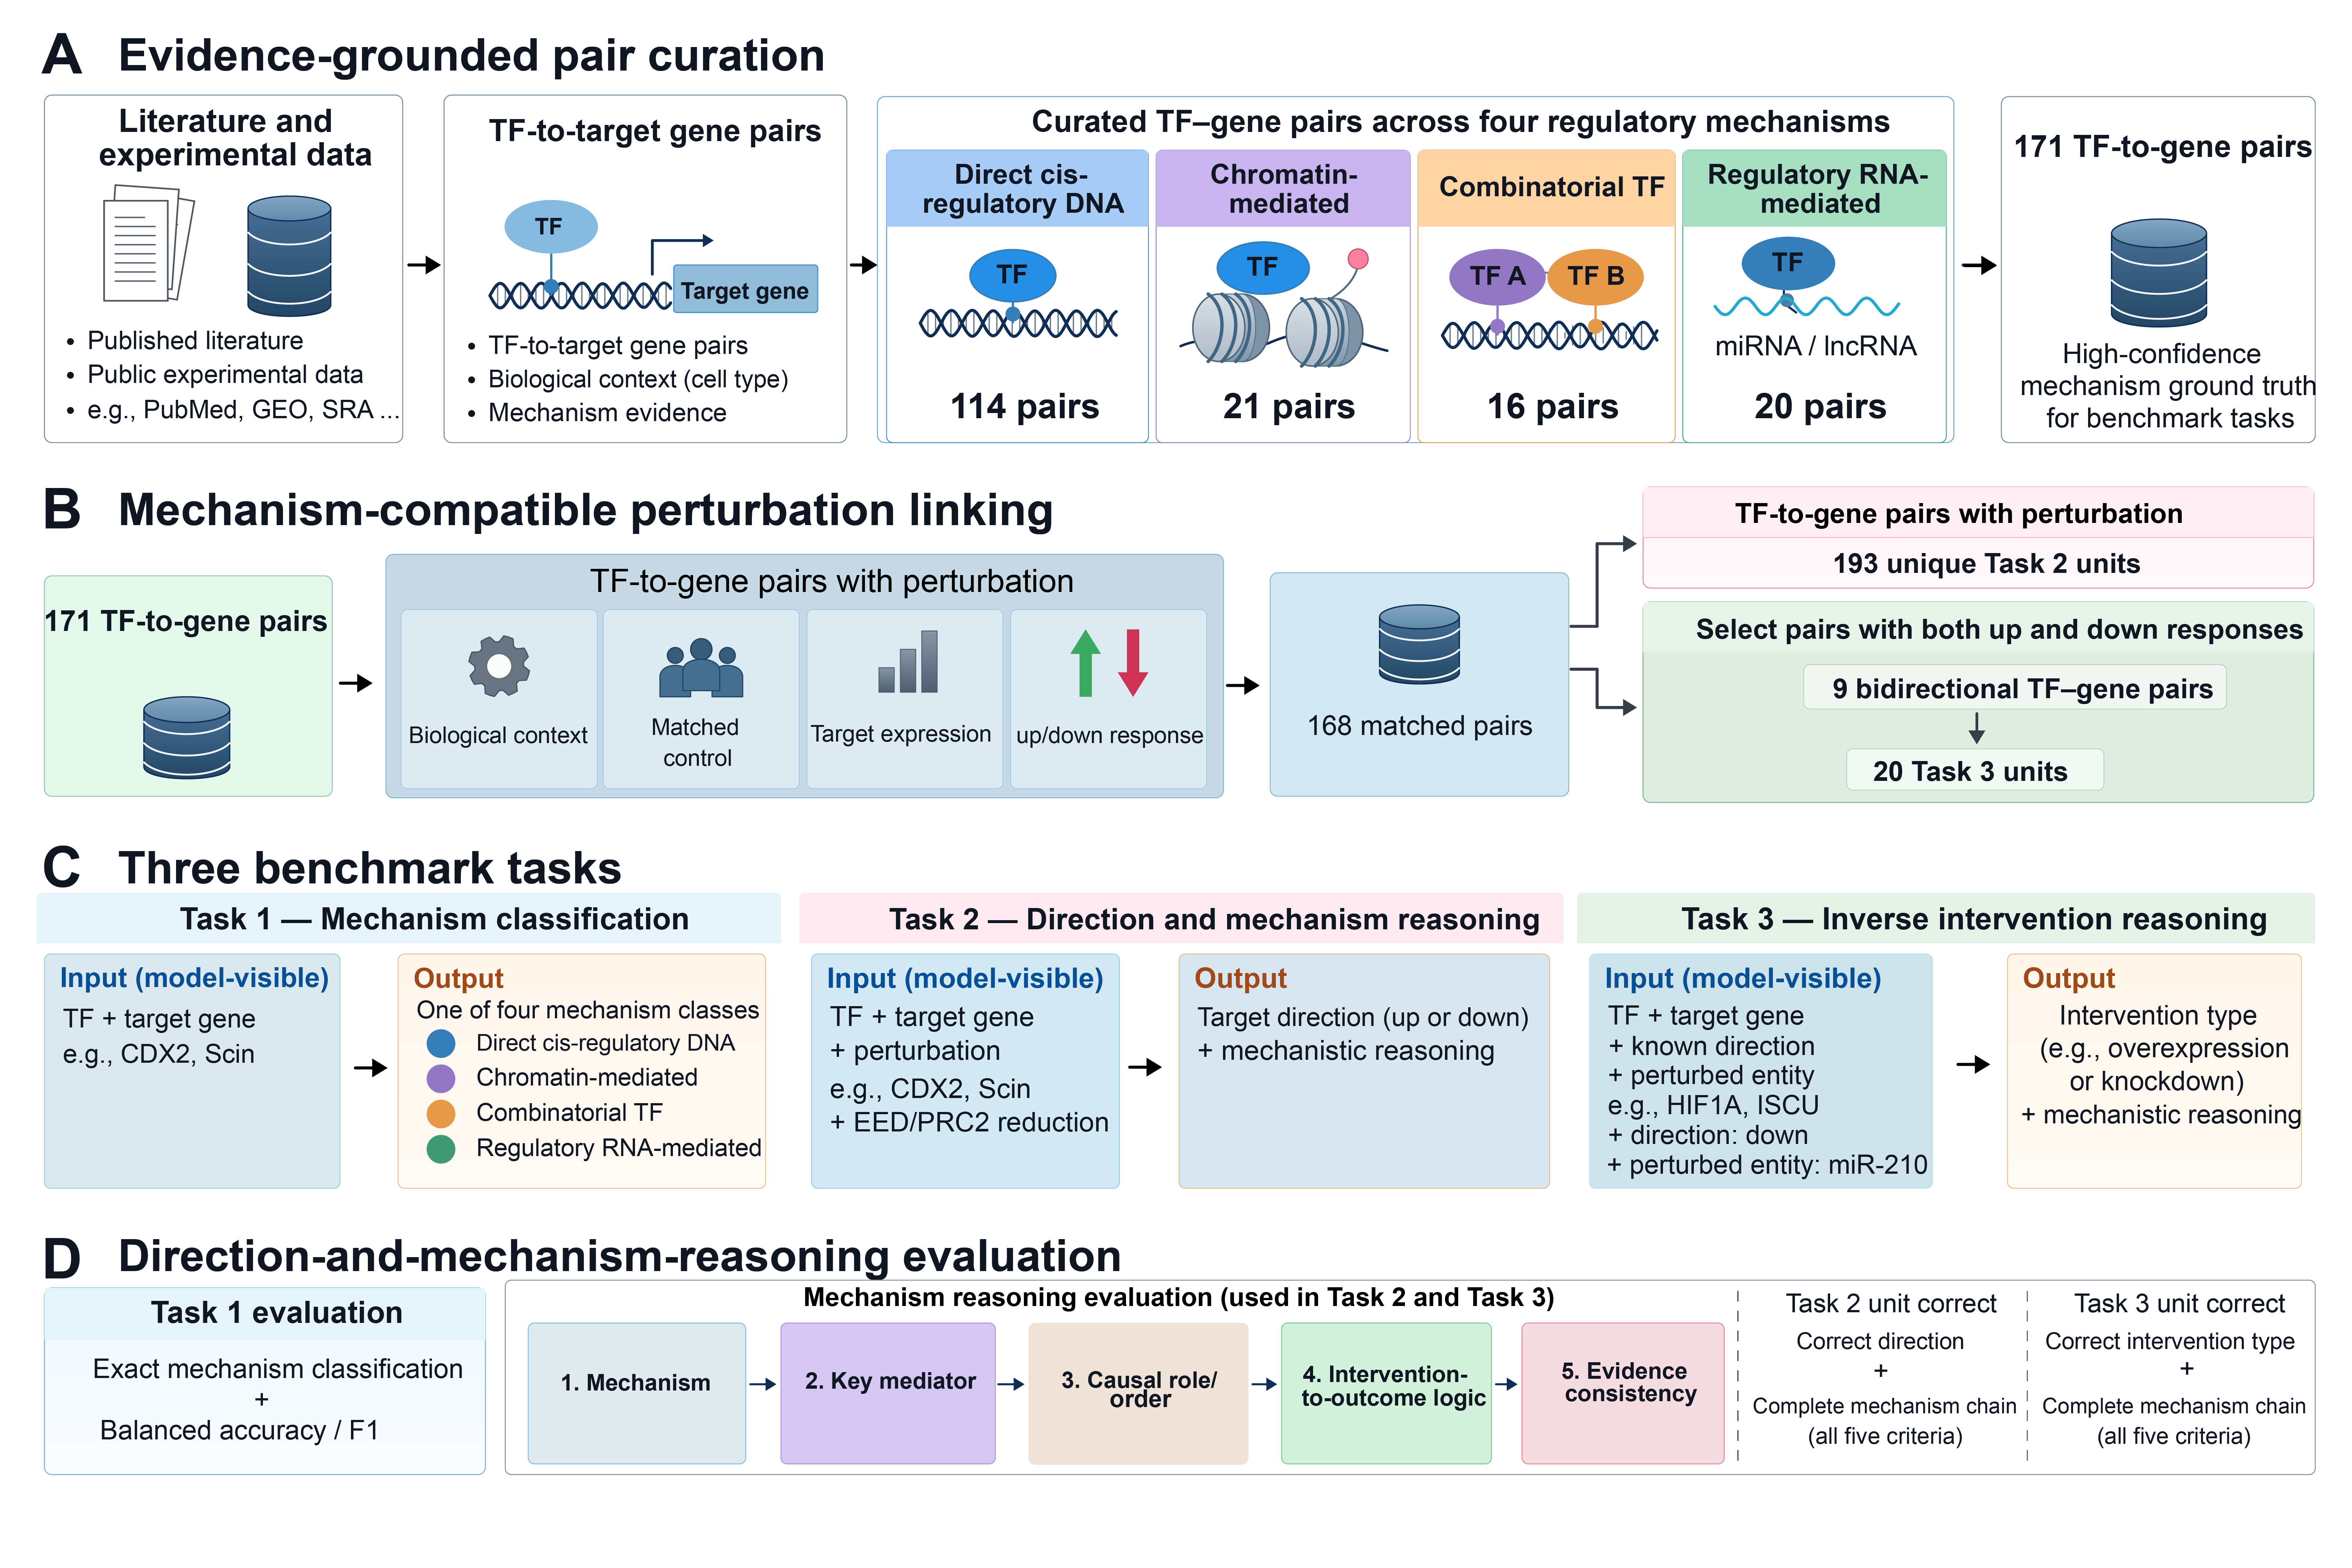
\includegraphics[width=0.85\linewidth]{figs/Fig_1-01.png}
  \captionsetup{skip=2pt}
  \caption{Construction and evaluation of MeBench.
  The benchmark contains 171 accepted TF-to-gene pairs, 193 evaluation units in Task 2, and 20 Task 3 units based on different perturbation types for the same TF-to-gene pairs. The three tasks assess mechanism identification, forward mechanistic reasoning and inverse mechanistic reasoning.}
  \label{fig:benchmark_overview}
\end{figure}



Task 1 includes 171 TF-to-gene pairs: 114 assigned to direct cis-regulatory DNA, 21 to chromatin-mediated regulation, 16 to combinatorial TF regulation and 20 to regulatory RNA-mediated regulation. Task 2 comprises 193 evaluation units covering 168 TF-to-gene pairs, including 112 direct cis-regulatory DNA, 20 chromatin-mediated, 35 combinatorial TF and 26 regulatory RNA-mediated units. Of these, 167 are labelled down and 26 up. Task 3 contains 20 evaluation units across nine TF-to-gene pairs, with 10 units each for combinatorial TF and regulatory RNA-mediated regulation (Figure~\ref{fig:unit_number}).

\begin{figure}[!htbp]
  \centering
  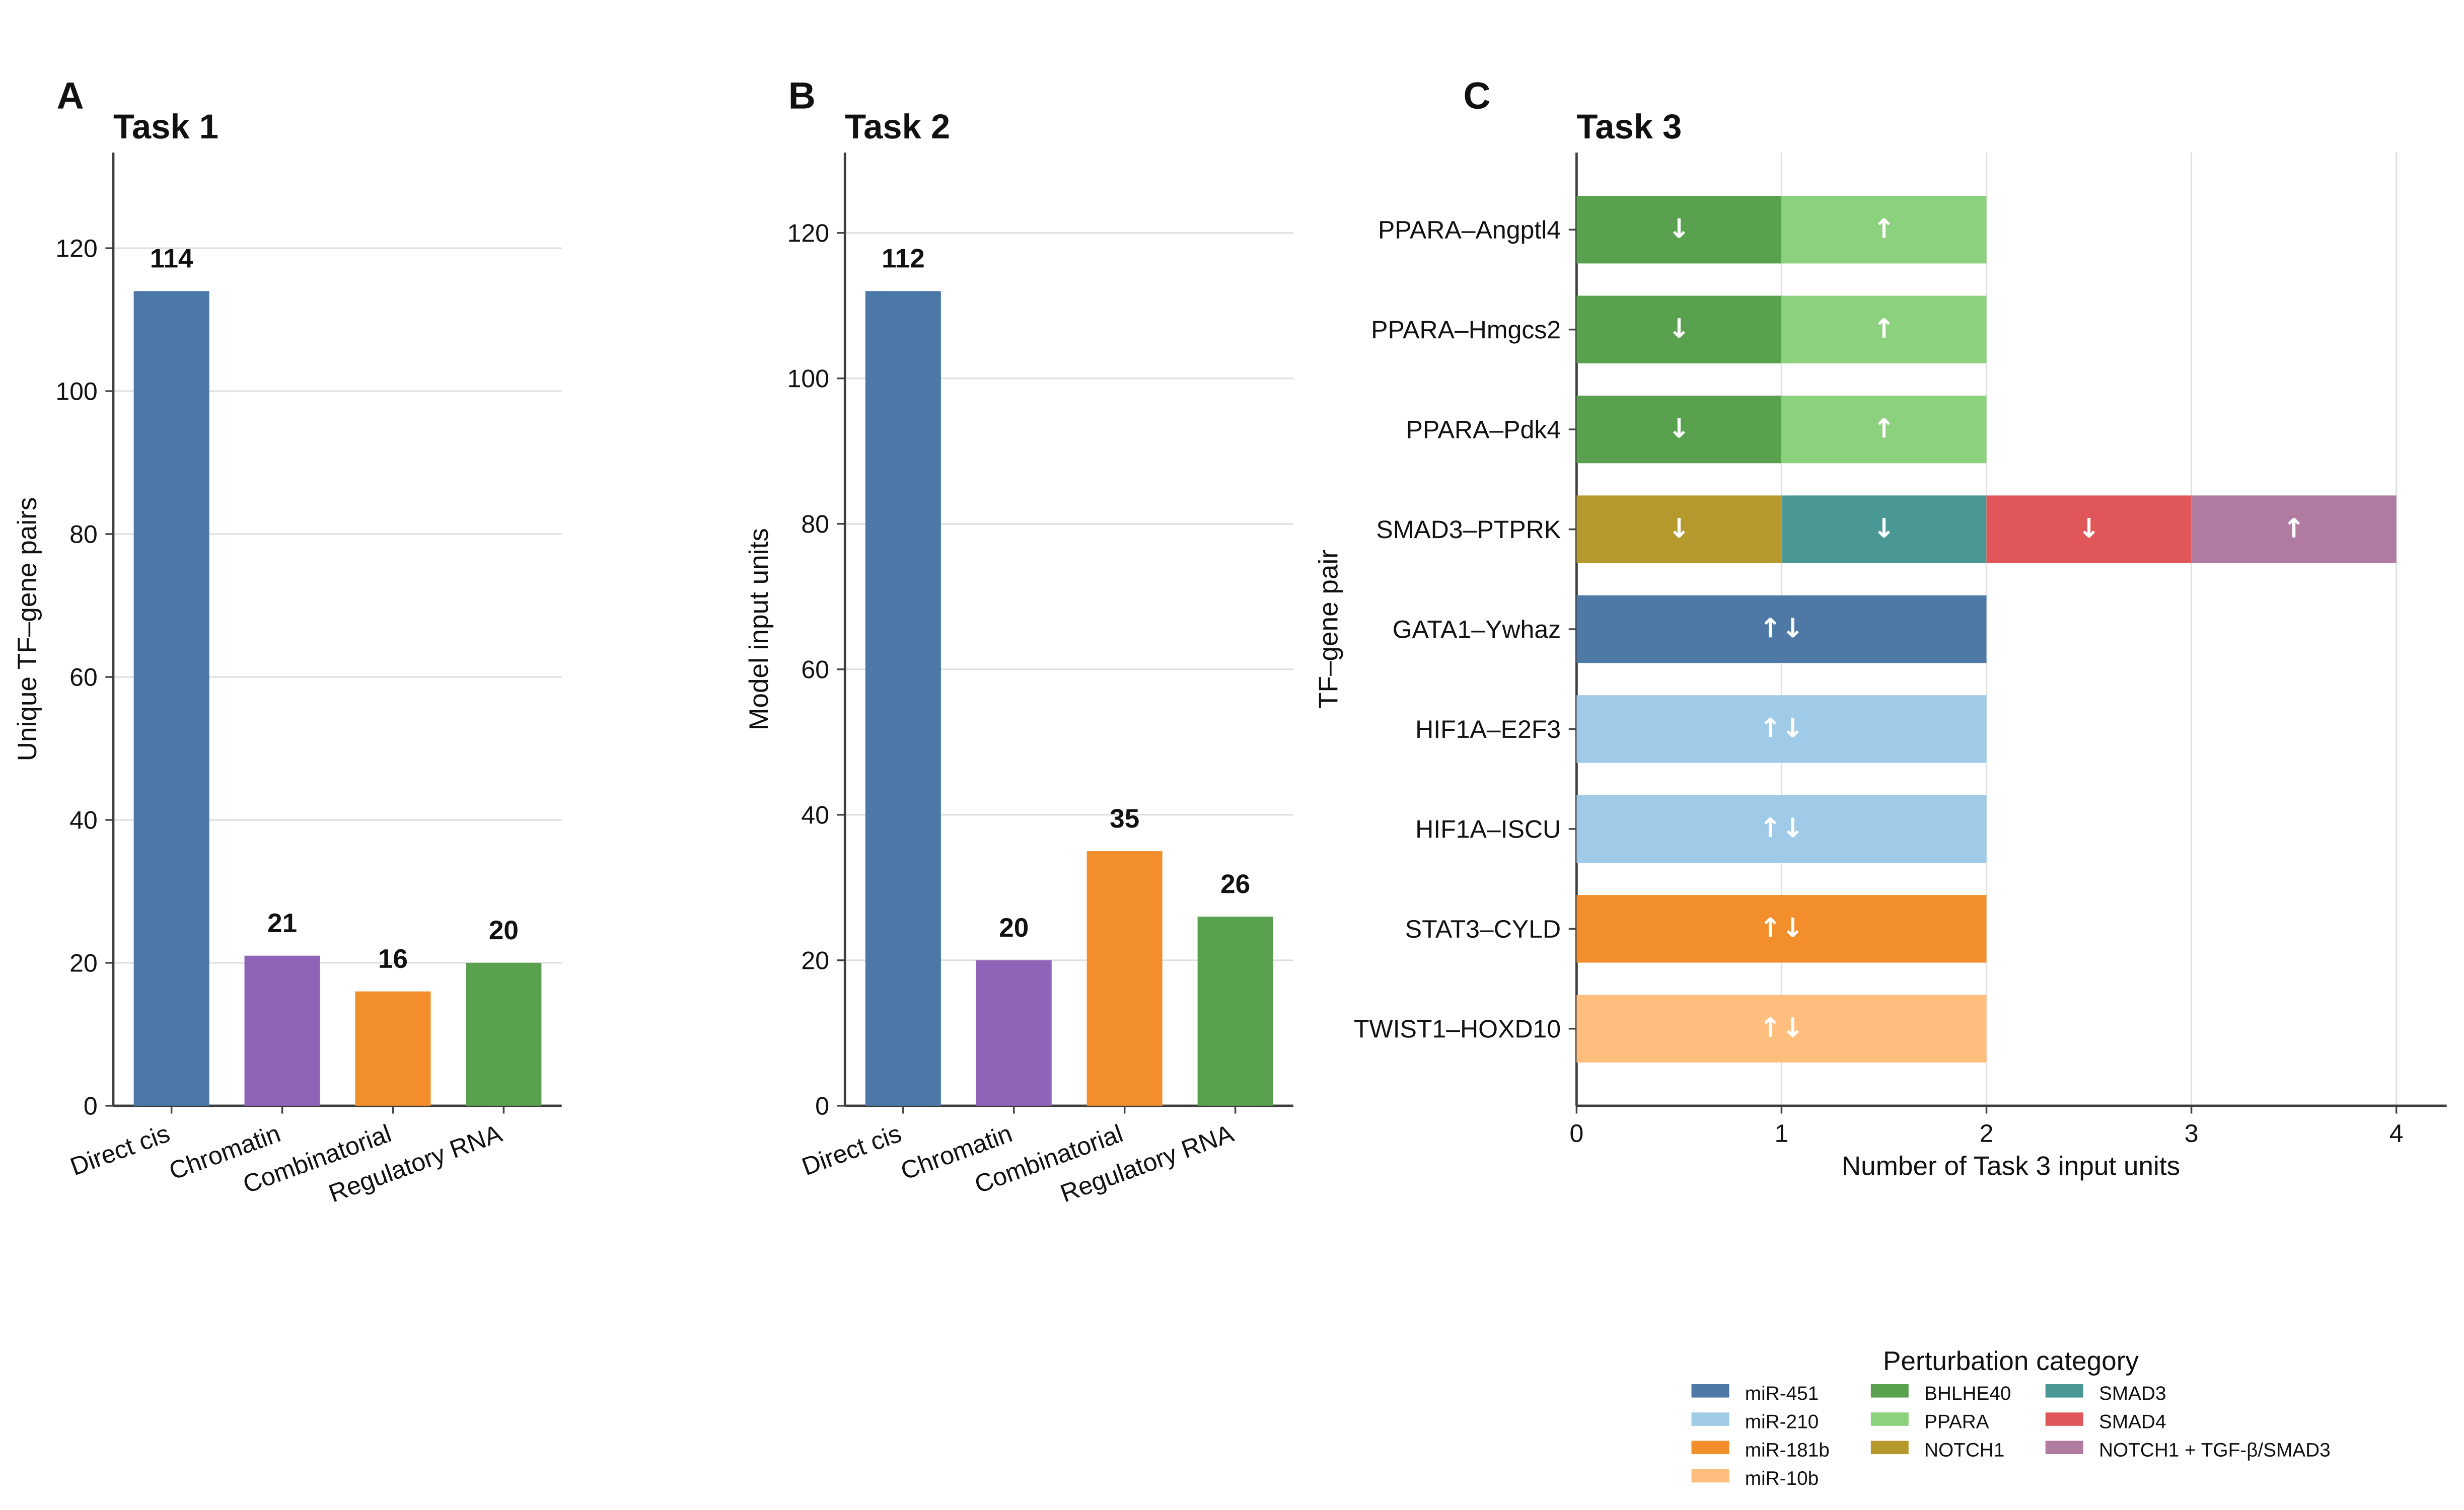
\includegraphics[width=0.82\linewidth]{figs/Fig_2.png}
  \captionsetup{skip=2pt}
  \caption{Number of the evaluation units in each task.
  (A) Distribution of 171 unique TF--gene pairs across four regulatory mechanisms in Task 1.
  (B) Distribution of 193 input units across four regulatory mechanism categories in Task 2.
  (C) Composition of 20 input units spanning nine TF--gene pairs in Task 3.}
  \label{fig:unit_number}
\end{figure}



\subsection{Benchmarking methods}

Task 1 provides only the TF and target gene and asks models to select one of the four mechanism labels. Biological context, perturbations, expression measurements, source information and curator notes are withheld. Task 2 provides TF, target gene, and the perturbation and asks for an up/down prediction and one concise mechanistic reasoning in natural language. Task 3 supplies the TF, target, response direction, and perturbed entity, and requests an intervention type and reasoning. The nine pairs have documented responses in both directions under different perturbations (Figure~\ref{fig:task_input}).

\begin{figure}[!htbp]
  \centering
  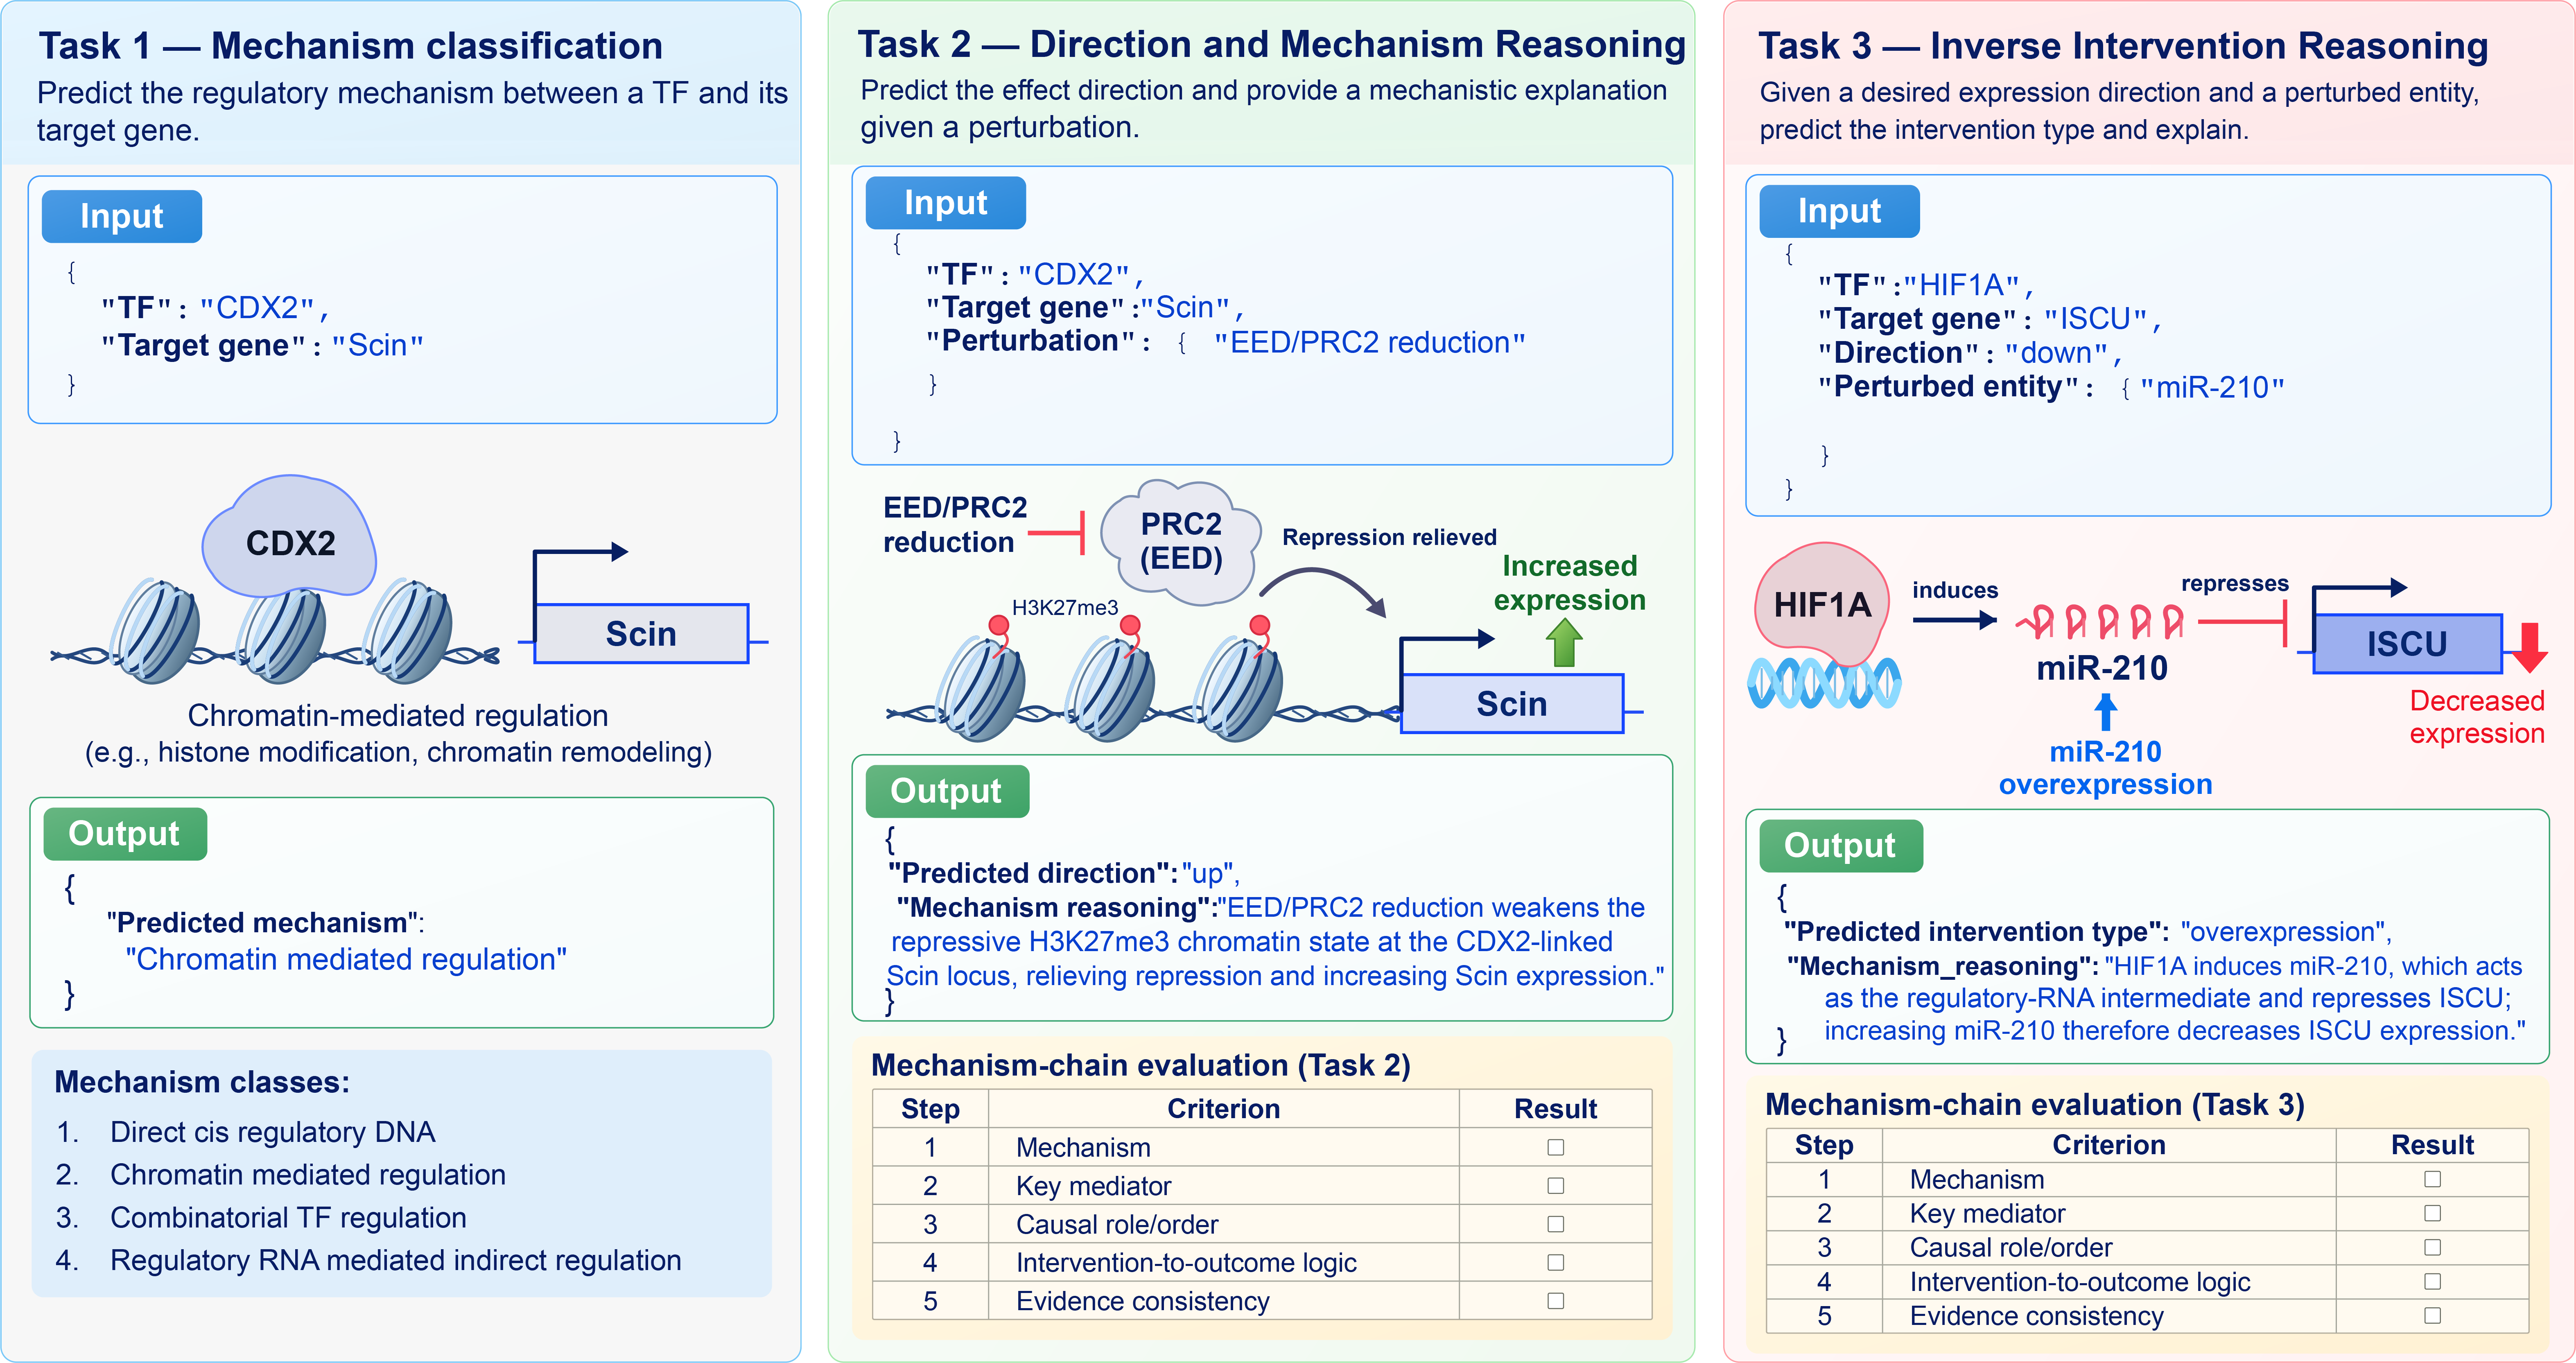
\includegraphics[width=0.85\linewidth]{figs/Fig_3.png}
  \captionsetup{skip=2pt}
  \caption{Examples of tasks' inputs and outputs.}
  \label{fig:task_input}
\end{figure}






We assessed models’ mechanistic reasoning using five criteria: mechanism correctness, mediator correctness, causal role and order, intervention-to-outcome logic, and evidence consistency. Mechanism correctness assesses whether the reasoning identifies the experimentally supported regulatory category for the TF–gene relationship. Mediator correctness evaluates whether it identifies the key component required for that mechanism, such as a chromatin regulator, partner TF, or regulatory RNA. Causal role and order assesses whether the reasoning correctly assigns activating or repressive functions to the relevant components and places them in the appropriate causal sequence. Intervention-to-outcome logic evaluates whether the explanation correctly connects the supplied perturbation in Task 2, or the inferred intervention in Task 3, to the target gene’s response direction. Finally, evidence consistency checks whether the reasoning makes claims that conflict with the curated experimental evidence, including incorrect molecular interactions, functional roles, or regulatory effects. The mechanistic reasoning passes the full-chain evaluation only when all five criteria are satisfied ~\eqref{eq:mechanism_scoring}. 

\begin{equation}
\label{eq:mechanism_scoring}
C_i = \prod_{k=1}^{5} r_{ik},
\qquad
J_i^{(2)} = \mathbb{1}\!\left[\hat{y}_i = y_i\right] C_i,
\qquad
J_i^{(3)} = \mathbb{1}\!\left[v(\hat{a}_i) \in A_i\right] C_i.
\end{equation}

Here, \(i\) indexes evaluation units and \(k\) indexes the five explanation criteria. The binary judgment \(r_{ik}\) indicates whether unit \(i\) satisfies criterion \(k\), and \(C_i=1\) only when all five criteria are met. For Task 2, \(y_i\) and \(\hat{y}_i\) denote the reference and predicted target-gene response directions, respectively. For Task 3, \(\hat{a}_i\) denotes the predicted intervention type, \(v\) is the string-normalization function used by the scorer, and \(A_i\) contains the accepted intervention types for the supplied entity and response direction, with each reference type normalized using \(v\). The indicator function \(\mathbb{1}[\cdot]\) equals 1 when its condition is satisfied and 0 otherwise. For each task \(t \in \{2,3\}\), we calculate joint accuracy as the mean of \(J_i^{(t)}\) across that task's evaluation units. We also report the pass rate for each criterion, the full-chain pass rate, and the mean score across the five criteria. Each evaluation unit receives equal weight, without adjustment for the number of units associated with each TF-to-gene pair.


The prompts for the five text-only systems define all four regulatory mechanism classes and instruct models to use the supplied information without external tools, retrieval or citations (Figure~\ref{fig:task_prompt}). The systems identify the regulatory mechanism in Task 1, predict the direction of change in target gene expression in Task 2, and infer the intervention type in Task 3. Tasks 2 and 3 also require the mechanistic reasoning supporting the prediction. Results are reported for GPT-6-Astra, Claude-Sonnet-5.5, Gemini-3.8-Flash, GLM-5.3-Flash, Grok-4.6, and Biomni as means over four recorded runs. The five text-only systems use closed-book prompts; Biomni is a tool-augmented agent, so its results describe a different access setting. Five-axis judgments use cross-model evaluation. All authors discussed and agreed on the interpretation of the results, and author spot checks covered all five scoring dimensions. These internal checks do not replace independent blinded validation (Appendix~\ref{app:protocol}). 










\begin{figure}[H]
  \centering
  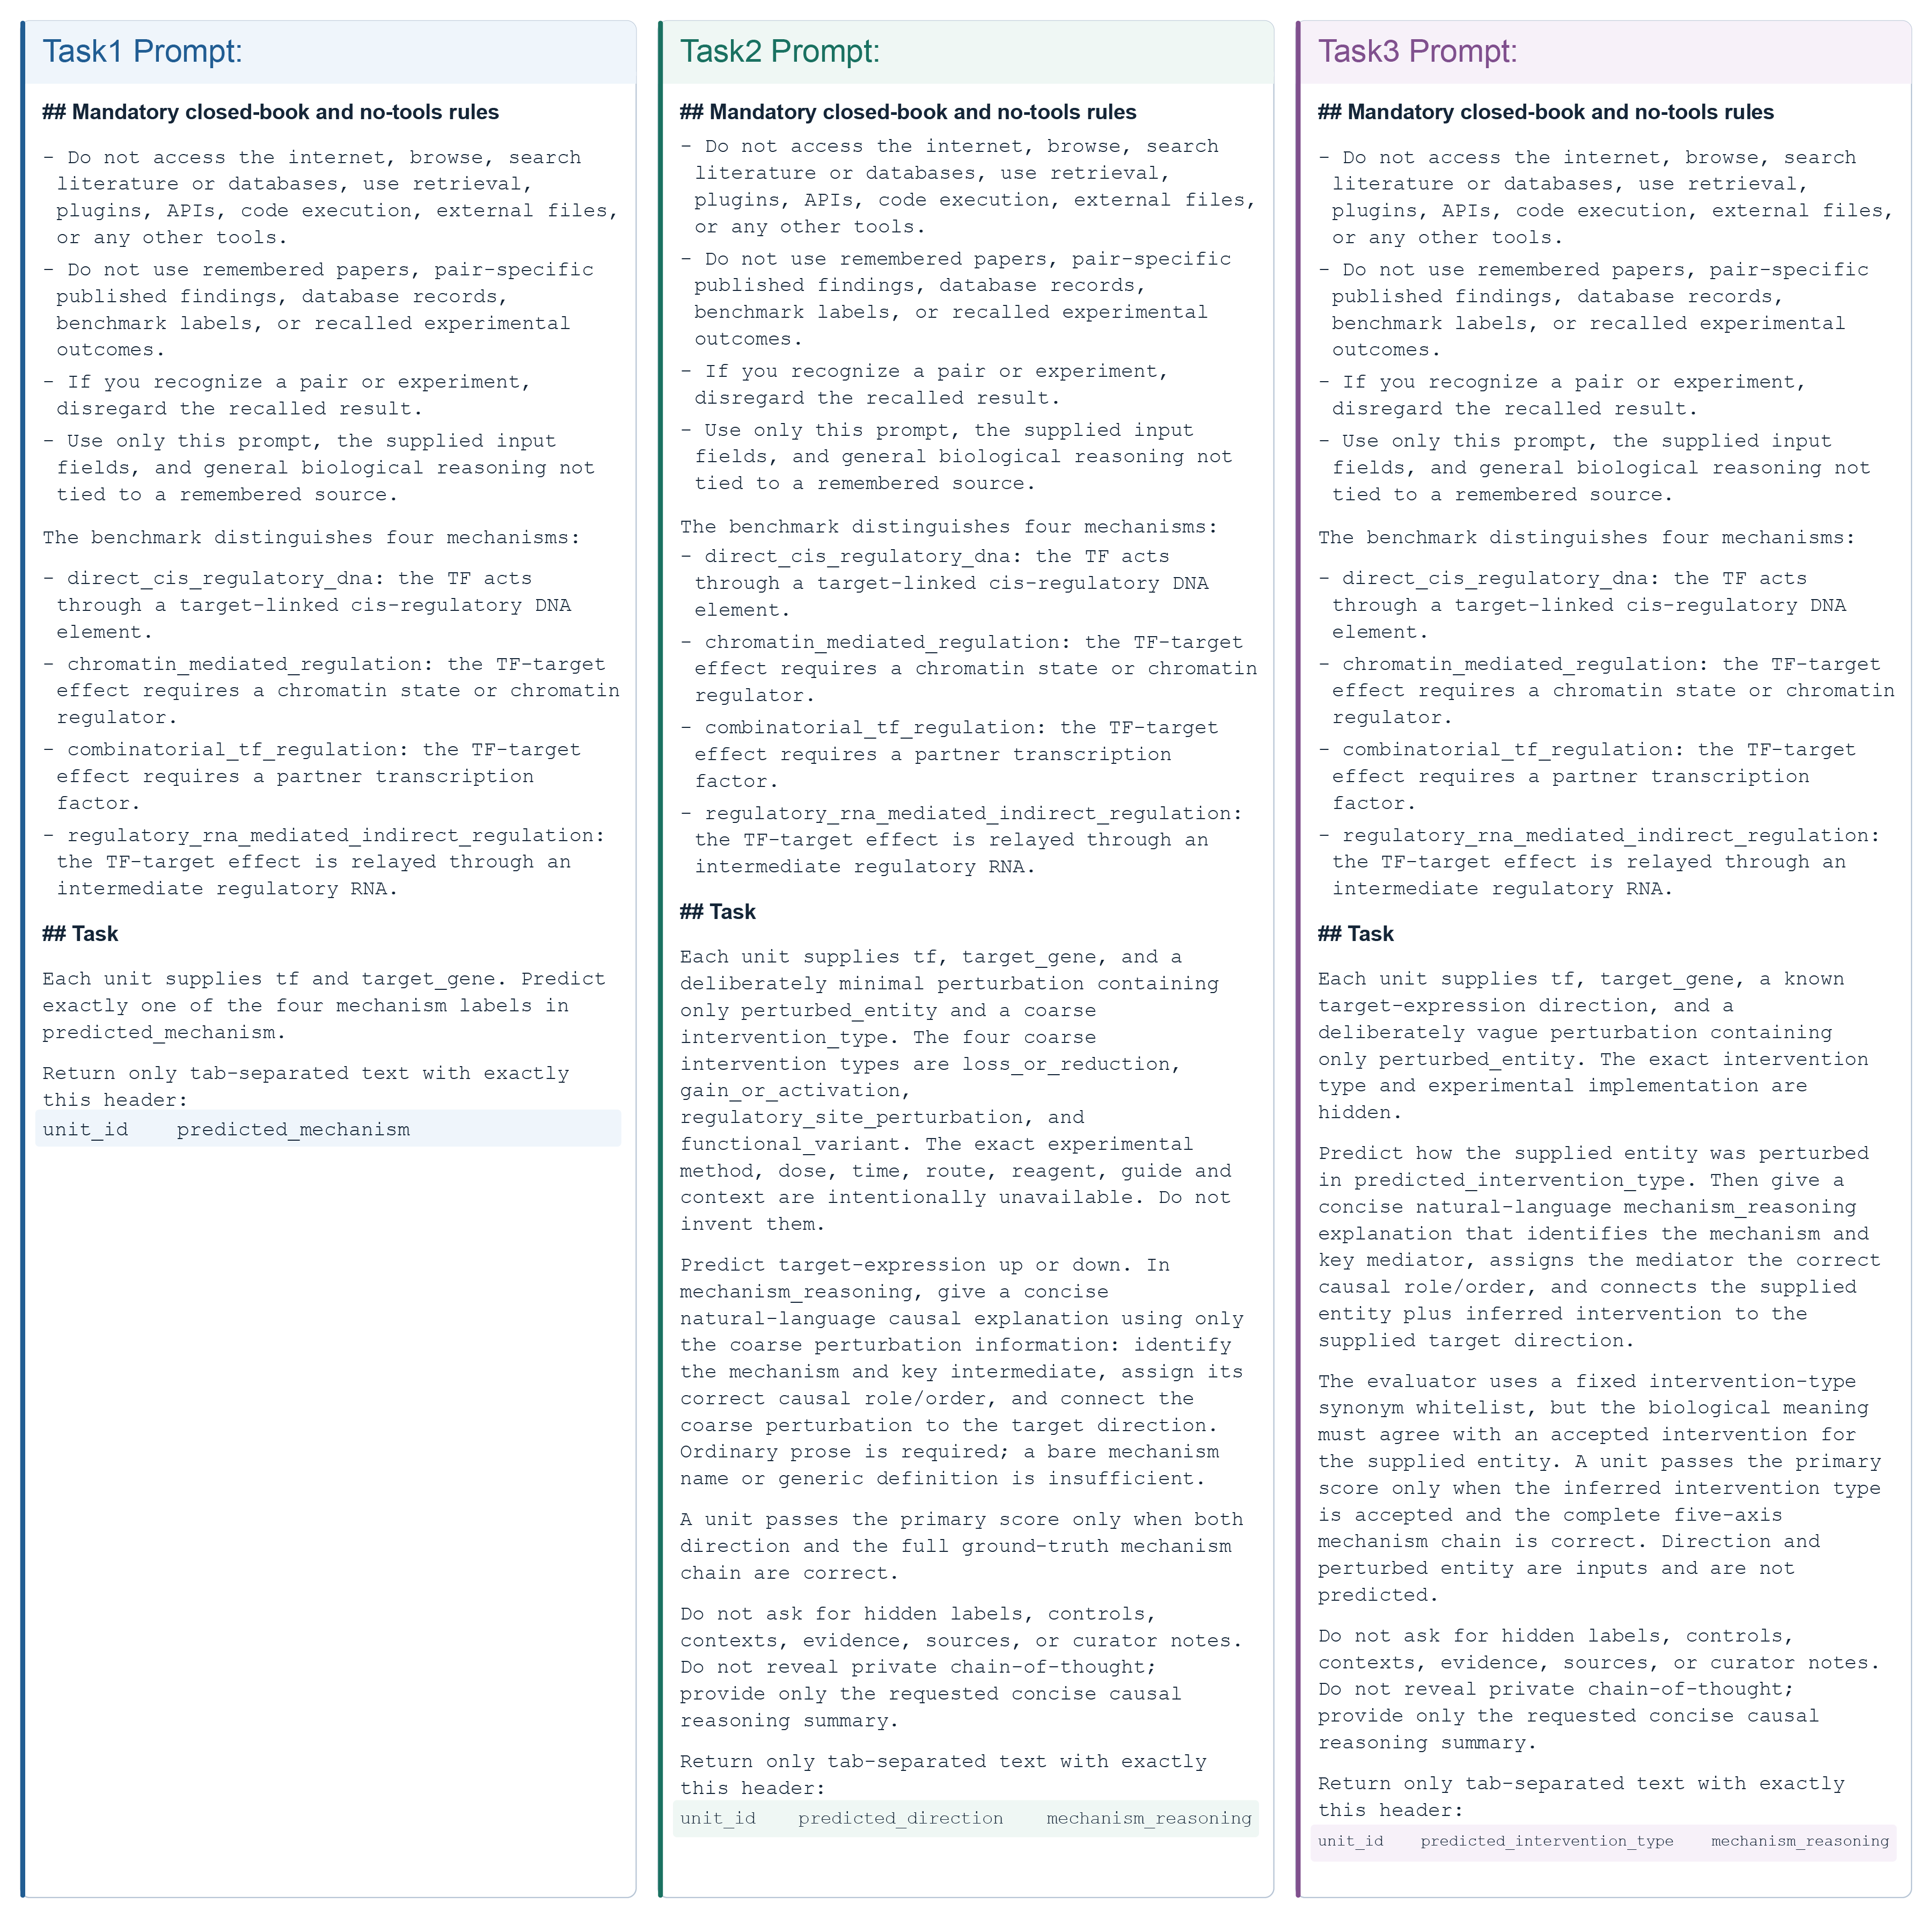
\includegraphics[width=0.85\linewidth]{figs/MeBench_task_prompts.png}
  \captionsetup{skip=3pt}
  \caption{Prompts for each task.}
  \label{fig:task_prompt}
\end{figure}
